%travail_proxy
\subsection{Procurateur}
\begin{figure}[h]
\begin{center}
    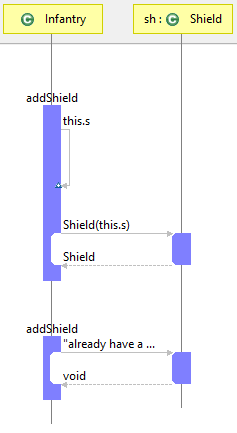
\includegraphics[width=11cm]{diagSeqProxy}
\end{center}
    \caption{Diagramme de séquence du pattern procurateur}
    \label{sequence-procurateur}
\end{figure}

Afin de contrôler les actions demandées par le client sur le soldat (comme par exemple l'ajout d'une nouvelle arme), nous avons appliqué le pattern \emph{Procuration}, voir la figure \vref{sequence-procurateur}, qui fournit au client une représentation "augmentée" de l'objet soldat, et qui aura pour rôle de contrôler, lors de l'ajout d'une arme sur un soldat, si le soldat possède déjà cette arme ou non.

Nous avons donc créé une interface \emph{Soldier} contenant deux méthodes permettant d'ajouter des armes : \emph{addShield} et \emph{addSword}. Cette interface étend l'interface plus générale \emph{SoldierInt}. 
Les classes \emph{Infantry} et \emph{Horseman} ont quand à elle été dupliquées et implémentent l'interface \emph{Soldier}(nous avons par la suite intercalé une classe abstraite afin d'éviter la duplication de code).

Enfin, nous avons rajouté une durée de vie à nos armes avec la variable \emph{RESISTANCE} que nous avons placé dans nos classes d'armes. La résistance de l'arme diminue de 1 point à chaque utilisation (c'est-à-dire à chaque appel aux méthodes \emph{strike} ou de \emph{parry}).